\chapter{التركيب الضوئي}\label{ch:g12:photosynthesis}

ضع غصينًا من عشبة الماء مقلوبًا في جرة ماء تحت مصباح، فيرتفع من الساق
المقطوعة تيار من الفقاعات: هو الأكسجين، فقاعة كل بضع ثوان، أسرع إذا
قرّب المصباح، وينقطع إذا أطفئ. والغاز هو النصف المرئي من مسار يغذي كل
حيوان على الكوكب وجعل الهواء صالحًا للتنفس قبل ملياري سنة. وقد أعطاه
\cref{ch:g10:cell-metabolism} في سطر واحد: ثنائي أكسيد الكربون والماء،
مع الضوء، يصيران سكرًا وأكسجينًا. وهذا الفصل يفتح \omterm{def:g12:photosynthesis:chloroplast}{البلاستيدة الخضراء}
ويتابع طاقة فوتون إلى داخل رابطة كيميائية.

\section{البلاستيدة الخضراء}

\begin{definition}[البلاستيدة الخضراء]\label{def:g12:photosynthesis:chloroplast}
\emph{البلاستيدة الخضراء}\index{بلاستيدة خضراء} \omterm{def:g10:cells-common-unit:organelle}{عضية} \omterm{def:g10:cell-metabolism:autotrophy}{التركيب الضوئي}:
جسم عدسي الشكل طوله نحو \qty{5}{\micro m}، يحده غشاء مضاعف، ويحوي
سائلًا هو \emph{الحشوة}، تقع فيه أكداس من أكياس غشائية مسطحة هي
\emph{التيلاكويدات}\index{تيلاكويد}. وأغشية التيلاكويد تحمل الأصبغة
--- \emph{اليخضور} a وb، وهما أخضران، والكاروتينات البرتقالية ---
وتحمل \omterm{def:g10:chemistry-of-life:families}{البروتينات} التي تحوّل طاقة الضوء؛ أما الحشوة فتحمل \omterm{def:g11:enzymes-and-phenotype:enzyme}{الإنزيمات} التي
تبني السكر. وتحوي \omterm{def:g10:cells-common-unit:cell}{خلية} الورقة عشرات \omterm{def:g10:cells-common-unit:organelle}{البلاستيدات الخضراء}، ويحوي
الميليمتر المربع من الورق نحو نصف مليون.
\end{definition}

\begin{omfigure}
\begin{tikzpicture}
  \node[anchor=south west, inner sep=0] (img) at (0,0)
    {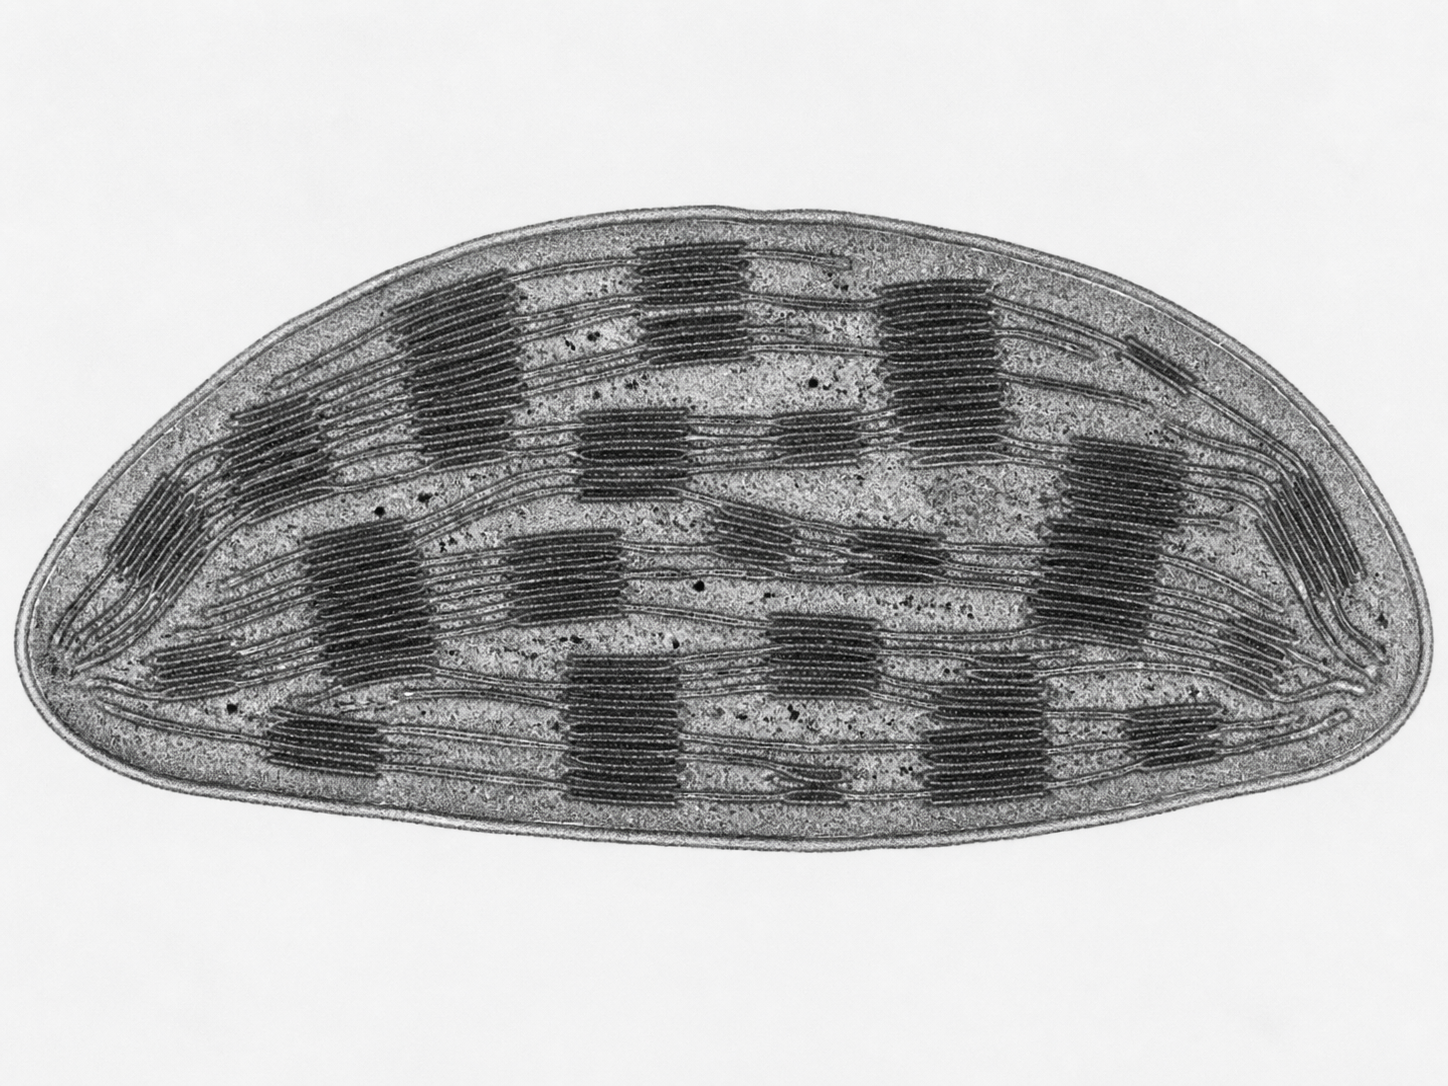
\includegraphics[width=0.5\linewidth]{images/book2/ai/g12-photo-chloroplast-tem.png}};
  \begin{scope}[x={(img.south east)}, y={(img.north west)},
      every node/.style={font=\small}]
    \draw[omDef, thick] (0.10,0.50) -- (-0.04,0.80) node[left, align=right] {غلاف\\ مضاعف};
    \draw[omDef, thick] (0.47,0.72) -- (0.47,1.06) node[above] {تيلاكويدات مكدسة (غرانوم)};
    \draw[omDef, thick] (0.62,0.42) -- (1.04,0.20) node[right] {الحشوة};
    \draw[omDef, thick] (0.80,0.60) -- (1.04,0.75) node[right, align=left] {أغشية تصل\\ بين الأكداس};
  \end{scope}
\end{tikzpicture}

{\small \omterm{def:g12:photosynthesis:chloroplast}{بلاستيدة خضراء} في المجهر الإلكتروني: الغلاف المضاعف، والحشوة،
وأغشية \omterm{def:g12:photosynthesis:chloroplast}{التيلاكويد} مكدسة في غرانا، حيث تجلس الأصبغة. فالضوء يلتقط في
الأغشية؛ والسكر يبنى في السائل حولها.}
\end{omfigure}

\begin{proposition}[أي ضوء يستعمل]\label{prop:g12:photosynthesis:spectrum}
اليخضور يمتص الضوء الأزرق والأحمر امتصاصًا قويًا ولا يكاد يمتص الأخضر
--- ولهذا كانت الأوراق خضرًا. \omterm{def:g10:cell-metabolism:autotrophy}{والتركيب الضوئي} تقوده الأطوال الموجية
التي تمتصها الأصبغة: فمعدله، مقيسًا بدلالة طول الموجة (وهو \emph{طيف
الفعل})، يرتفع وينخفض مع امتصاص الأصبغة، بذروتين في الأزرق والأحمر
وحضيض في الأخضر.
\end{proposition}
\begin{proof}[شواهد]
وضع إنغلمان (سنة 1882) خيطًا من طحلب أخضر في قطرة ماء فيها جراثيم
تسبح نحو الأكسجين، وأسقط طيفًا على طول الخيط عبر المجهر: فتجمعت
الجراثيم حول القطع المضاءة بالأزرق وبالأحمر، وتحاشت الأخضر --- إذ كان
الأكسجين يتحرر حيث سقط هذان اللونان. والقياس الحديث لخرج الأكسجين تحت
مصابيح ملونة يعطي المنحني نفسه، وهو يطابق طيف امتصاص الأصبغة
المستخلصة.
\end{proof}

\begin{omfigure}
\begin{tikzpicture}
\begin{axis}[
  width=0.88\linewidth, height=5.8cm,
  axis x line=bottom, axis y line=left,
  xmin=400, xmax=700, ymin=0, ymax=110,
  xlabel={طول الموجة (nm)}, ylabel={\% من الأعظم},
  xlabel style={font=\small, at={(axis description cs:0.5,-0.12)}, anchor=north},
  ylabel style={font=\small},
  tick label style={font=\small}, xtick={400,450,500,550,600,650,700}, ytick={0,50,100},
  legend style={at={(0.5,-0.3)}, anchor=north, legend columns=2, font=\small, draw=none},
]
\addplot[thick, omMeth, smooth] coordinates {(400,70) (430,100) (450,75) (480,35) (500,15) (550,8) (600,15) (640,45) (665,90) (680,70) (700,10)};
\addplot[thick, omThm, dashed, smooth] coordinates {(400,65) (430,85) (450,80) (480,55) (500,35) (550,25) (600,35) (640,60) (665,95) (680,100) (700,20)};
\legend{{الامتصاص عند أصبغة الورقة}, {معدل التركيب الضوئي (طيف الفعل)}}
\end{axis}
\end{tikzpicture}

{\small امتصاص الضوء عند أصبغة ورقة مستخلصة، ومعدل \omterm{def:g10:cell-metabolism:autotrophy}{التركيب الضوئي} عند
الورقة، بدلالة طول الموجة. وكلاهما يبلغ ذروته في الأزرق والأحمر وينخفض
في الأخضر: فالضوء الذي يقود \omterm{def:g10:cell-metabolism:autotrophy}{التركيب الضوئي} هو الضوء الذي تمتصه
الأصبغة.}
\end{omfigure}

\section{المرحلة الضوئية: الماء يشق والطاقة تخزن}

\begin{proposition}[ما يجري في التيلاكويدات]\label{prop:g12:photosynthesis:lightphase}
في أغشية \omterm{def:g12:photosynthesis:chloroplast}{التيلاكويد}، في الضوء، تقع ثلاثة أمور معًا:
\begin{itemize}
  \item جزيئات الماء \emph{تشق}: فيتحرر أكسجينها على صورة
        $\mathrm{O_2}$ --- فأكسجين \omterm{def:g10:cell-metabolism:autotrophy}{التركيب الضوئي} آت من الماء لا من
        ثنائي أكسيد الكربون --- ويحتفظ بهيدروجينها إلكترونات
        وبروتونات؛
  \item وطاقة الفوتونات الممتصة تستعمل في تحميل تلك الإلكترونات على
        جزيء حامل هو \emph{NADP المرجَع}، وستستعمله الحشوة مصدرًا
        للهيدروجين؛
  \item والطاقة نفسها تقود تركيب \emph{ATP}.
\end{itemize}
فالمرحلة الضوئية تحوّل الضوء إذن إلى ناتجين كيميائيين، هما ATP وNADP
المرجَع، وتحرر الأكسجين ناتجًا ثانويًا. ولا شأن لثنائي أكسيد الكربون
بها.
\end{proposition}
\begin{proof}[شواهد]
أضاء هيل (سنة 1937) بلاستيدات خضراء معزولة في ماء مع متلقٍّ اصطناعي
للإلكترونات وبلا ثنائي أكسيد الكربون: فحررت الأكسجين وأرجعت المتلقي.
فتحرر الأكسجين يحتاج ضوءًا وماء لا $\mathrm{CO_2}$، وهو مقترن بنقل
الإلكترونات. وأمدّ روبن وكامن (سنة 1941) طحالب بماء يحوي النظير الثقيل
$^{18}$O: فكان الأكسجين المتحرر ثقيلًا؛ وحين أمدّاها بثنائي أكسيد
كربون ثقيل وماء عادي لم يكن كذلك. فالأكسجين آت من الماء.
\end{proof}

\begin{omfigure}
\begin{tikzpicture}[font=\small, >=Stealth,
  b/.style={draw, rounded corners, align=center, minimum height=1.0cm}]
  % thylakoid box
  \node[b, fill=omMeth!15, text width=3.6cm, minimum height=3.2cm] (thy) at (0,0) {};
  \node[anchor=north, font=\small\bfseries] at (thy.north) {أغشية التيلاكويد};
  \node[font=\small, align=center] at (0,-0.1) {ضوء يمتصه\\ اليخضور};
  % stroma box
  \node[b, fill=omDef!10, text width=3.6cm, minimum height=3.2cm] (str) at (6.4,0) {};
  \node[anchor=north, font=\small\bfseries] at (str.north) {الحشوة};
  \node[font=\small, align=center] at (6.4,-0.1) {دورة كالفن:\\ $\mathrm{CO_2}$ يثبَّت\\ في السكر};
  % inputs/outputs
  \draw[->, thick, omProp] (-3.2,1.0) -- (thy.west |- 0,1.0) node[pos=0, left, omProp] {الضوء};
  \draw[->, thick] (-3.2,-0.6) -- (thy.west |- 0,-0.6) node[pos=0, left] {$\mathrm{H_2O}$};
  \draw[->, thick] (thy.south) -- ++(0,-1.0) node[below] {$\mathrm{O_2}$ يتحرر};
  \draw[->, thick, omThm] (thy.east |- 0,0.7) -- (str.west |- 0,0.7) node[midway, above] {ATP};
  \draw[->, thick, omThm] (thy.east |- 0,-0.3) -- (str.west |- 0,-0.3) node[midway, above] {NADP المرجَع};
  \draw[->, thick, gray] (str.west |- 0,-1.1) -- (thy.east |- 0,-1.1) node[midway, below, font=\scriptsize] {الحاملان يعودان};
  \draw[->, thick] (9.6,0.6) -- (str.east |- 0,0.6) node[pos=0, right] {$\mathrm{CO_2}$};
  \draw[->, thick] (str.east |- 0,-0.6) -- (9.6,-0.6) node[right] {سكر};
\end{tikzpicture}

{\small مرحلتا \omterm{def:g10:cell-metabolism:autotrophy}{التركيب الضوئي}. في أغشية \omterm{def:g12:photosynthesis:chloroplast}{التيلاكويد}، يشق الضوء الماء
ويحرر الأكسجين ويشحن حاملين، هما ATP وNADP المرجَع. وفي الحشوة يدفع
الحاملان ثمن تثبيت ثنائي أكسيد الكربون في السكر. فالمرحلة الأولى تحتاج
الضوء؛ والثانية لا تحتاج إلا نواتجه.}
\end{omfigure}

\section{مرحلة الكربون: بناء السكر}

\begin{proposition}[دورة كالفن]\label{prop:g12:photosynthesis:calvin}
في الحشوة، يوصل ثنائي أكسيد الكربون، جزيئًا في كل مرة، بسكر خماسي
الكربون موجود أصلًا، وذلك بأوفر \omterm{def:g11:enzymes-and-phenotype:enzyme}{إنزيم} على الأرض؛ والناتج السداسي
الكربون ينشق في الحال إلى جزيئين ثلاثيي الكربون، يرجعان --- باستعمال
ATP وNADP المرجَع الآتيين من المرحلة الضوئية --- إلى سكاكر ثلاثية
الكربون. ويعاد تدوير معظمها لتجديد المتلقي الخماسي الكربون، فتنغلق
\emph{دورة كالفن}\index{دورة كالفن}؛ ويغادر واحد من كل ستة الدورة
مكسبًا صافيًا للنبات. فثلاث دورات، وثلاثة جزيئات $\mathrm{CO_2}$
تثبَّت، وتسعة ATP وستة NADP مرجَع تنفق: يصدَّر سكر ثلاثي الكربون واحد.
واثنان منه يصنعان غلوكوزًا.
\end{proposition}
\begin{proof}[شواهد]
أعطى كالفن (في خمسينيات القرن العشرين) طحالب ثنائي أكسيد كربون موسومًا
بالكربون المشع $^{14}$C بضع ثوان، وقتلها في كحول مغلي، وفصل جزيئاتها:
فبعد خمس ثوان كان الوسم في حمض ثلاثي الكربون واحد؛ وبعد ثلاثين، في
سكاكر ثلاثية الكربون وفي المتلقي الخماسي؛ وبعد دقائق، في السكروز
والنشاء. وقطع الضوء ترك المتلقي غير مجدَّد والحمض الثلاثي الكربون
يتراكم؛ وقطع $\mathrm{CO_2}$ ترك المتلقي يتراكم. فترتيب الظهور هو
ترتيب الدورة.
\end{proof}

\begin{omfigure}
\begin{tikzpicture}[font=\small, >=Stealth]
  \draw[thick, ->] (90:2.2) arc (90:-30:2.2);
  \draw[thick, ->] (-30:2.2) arc (-30:-150:2.2);
  \draw[thick, ->] (-150:2.2) arc (-150:-270:2.2);
  \node[draw, rounded corners, fill=omDef!12, align=center, font=\small] at (90:2.2) {متلقٍّ خماسي\\ الكربون ($\times 3$)};
  \node[draw, rounded corners, fill=omProp!15, align=center, font=\small] at (-30:2.2) {حمض ثلاثي الكربون\\ ($\times 6$)};
  \node[draw, rounded corners, fill=omMeth!15, align=center, font=\small] at (-150:2.2) {سكر ثلاثي الكربون\\ ($\times 6$)};
  \draw[->, thick] (3.6,2.2) -- (2.4,1.6) node[pos=0, right, align=left] {$3\,\mathrm{CO_2}$ تدخل};
  \draw[->, thick, omThm] (2.2,-2.4) -- (1.2,-2.0) node[pos=0, right, omThm, align=left] {6 ATP، و6 NADP مرجَع\\ من المرحلة الضوئية};
  \draw[->, thick, omThm] (-3.6,1.0) -- (-2.2,1.4) node[pos=0, left, omThm] {3 ATP};
  \draw[->, thick] (-2.4,-2.4) -- (-3.6,-3.2) node[anchor=north, align=center] {سكر ثلاثي الكربون واحد يغادر:\\ نصف غلوكوز};
  \node[font=\scriptsize, align=center] at (0,0) {خمسة من السكاكر الستة\\ تعيد بناء\\ المتلقيات الثلاثة};
\end{tikzpicture}

{\small \omterm{prop:g12:photosynthesis:calvin}{دورة كالفن}، محسوبة لثلاث دورات. ثلاثة جزيئات ثنائي أكسيد
الكربون تنضم إلى ثلاثة متلقيات خماسية الكربون؛ والنواتج الستة الثلاثية
الكربون ترجَع إلى سكاكر على حساب ATP وNADP المرجَع الآتيين من المرحلة
الضوئية؛ ويعاد تدوير خمسة من الستة إلى المتلقيات وواحد هو المكسب.}
\end{omfigure}

\begin{example}[حساب غلوكوز]\label{ex:g12:photosynthesis:bookkeeping}
يحتاج غلوكوز واحد إلى ست جزيئات من ثنائي أكسيد الكربون، أي إلى ست
دورات،
و18 جزيء ATP و12 جزيء NADP مرجَعًا، تمدها كلها المرحلة
الضوئية، وهي تشق 12 جزيء
ماء وتحرر ستة جزيئات أكسجين لصنعها. وحصيلته الصافية هي:
$6\,\mathrm{CO_2} + 12\,\mathrm{H_2O} \to \mathrm{C_6H_{12}O_6} +
6\,\mathrm{O_2} + 6\,\mathrm{H_2O}$،
وهي معادلة
\cref{ch:g10:cell-metabolism} الإجمالية، والماء الآن على الطرفين، إذ
إن الأكسجين المتحرر آت من الماء المشقوق لا من ثنائي أكسيد الكربون.
\end{example}

\begin{omfigure}
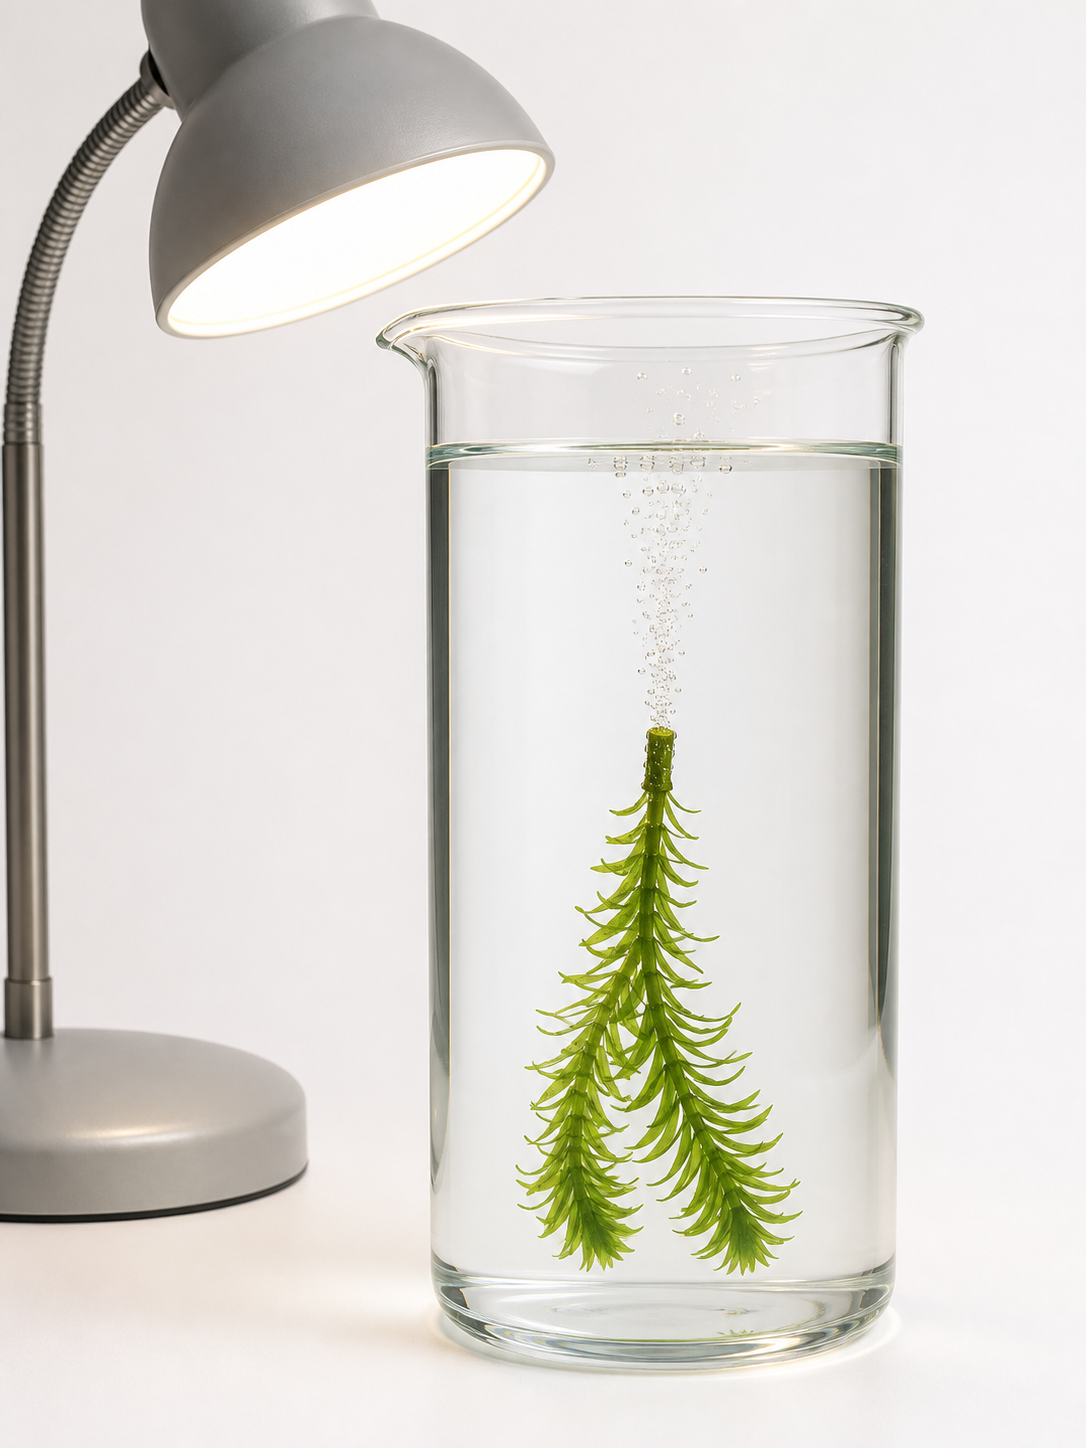
\includegraphics[width=0.34\linewidth]{images/book2/ai/g12-photo-elodea-bubbles.png}

{\small عشبة الماء تحت مصباح: الفقاعات الصاعدة من الساق المقطوعة هي
أكسجين المرحلة الضوئية. أحصها في الدقيقة، وحرّك المصباح، وغيّر لونه،
تقس معدل \omterm{def:g10:cell-metabolism:autotrophy}{التركيب الضوئي}.}
\end{omfigure}

\section{ماذا يصير السكر، وكم مقداره}

\begin{proposition}[مصائر الناتج]\label{prop:g12:photosynthesis:fates}
السكاكر الثلاثية الكربون المغادرة للدورة تركَّب، في \omterm{def:g12:photosynthesis:chloroplast}{البلاستيدة
الخضراء}، \emph{نشاءً}، وهو مخزن الورقة النهاري، أو تصدَّر إلى
\omterm{def:g10:cells-common-unit:cell}{السيتوبلازم} وتحوَّل \emph{سكروزًا}، وهو السكر الذي يحمله \omterm{prop:g12:plant-rooted-life:saps}{اللحاء}
(\cref{ch:g12:plant-rooted-life}). ومنها يصنع النبات كل ما سواها:
السيللوز للجدر، والدسم، و--- مع الآزوت والكبريت من التربة --- \omterm{def:g10:chemistry-of-life:families}{الحموض
الأمينية} \omterm{def:g10:universal-dna:nucleotide}{والنوكليوتيدات}. \omterm{def:g10:cell-metabolism:autotrophy}{فالتركيب الضوئي} مصدر طاقة النبات ومصدر مادته
العضوية كلها، ومصدر \omterm{def:g10:chemistry-of-life:mineral-organic}{المادة العضوية} كلها تقريبًا على الأرض، عبر السلاسل
الغذائية.
\end{proposition}
\admitted

\begin{example}[المردود، من الورقة إلى الكوكب]\label{ex:g12:photosynthesis:efficiency}
تسلّم الشمس الساطعة نحو \qty{1000}{W} في المتر المربع، منها
نحو 45\% في أطوال موجية تستطيع الأصبغة استعمالها؛ وتحوّل الورقة في
أحسن الأحوال نحو 5\% من ذلك إلى سكر في النهار، ويحوّل محصول، على مدى
موسم، 1\% إلى 2\% من ضوء الشمس الكلي إلى كتلة حية. ومع صغر الكسر، فإن
المجموع هائل: \omterm{def:g10:cell-metabolism:autotrophy}{فالتركيب الضوئي} يثبّت نحو
\qty{1e11}{t} من الكربون في السنة --- أي سُبع الكربون الذي في الجو ---
ويحرر الأكسجين الذي يستهلكه التنفس والحريق والصدأ.
\end{example}

\begin{method}[الاستدلال في تجربة تركيب ضوئي]\label{met:g12:photosynthesis:experiment}
\begin{enumerate}
  \item عيّن ما يقاس: الأكسجين المتحرر (المرحلة الضوئية)، أم ثنائي
        أكسيد الكربون المأخوذ أو السكر المتكون (مرحلة الكربون)، أم
        الكتلة الحية (الكل، مع الزمن).
  \item عيّن ما يغيَّر: الضوء (شدة، ولونًا)، أم ثنائي أكسيد الكربون، أم
        الحرارة، أم الماء --- وعلى أي مرحلة يعمل.
  \item وتذكر أن النبات يتنفس في الوقت نفسه: فخرج الأكسجين المقيس هو
        الإنتاج ناقص التنفس؛ وفي الظلام لا يظهر إلا التنفس
        (\cref{ch:g10:cell-metabolism}).
  \item وتتبع الوسوم: فالنظير $^{18}$O في الماء يظهر في الأكسجين؛ و$^{14}$C
        في ثنائي أكسيد الكربون يظهر في السكاكر، بترتيب الدورة.
\end{enumerate}
\end{method}

\begin{remark}[ضوء، ثم كيمياء]\label{rem:g12:photosynthesis:light}
الخطوة الوحيدة من \omterm{def:g10:cell-metabolism:autotrophy}{التركيب الضوئي} التي تحتاج الضوء هي الأولى: تحميل
الإلكترونات من الماء على حامل، مع تحرر الأكسجين. وكل ما بعدها --- صنع
ATP، وتثبيت ثنائي أكسيد الكربون، وبناء السكر --- كيمياء تستمر في
الظلام ما دام الحاملان باقيين، وسيديرها تنفس الفصل التالي في الاتجاه
المعاكس. \omterm{def:g12:photosynthesis:chloroplast}{فالبلاستيدة الخضراء} هي حيث يحوَّل ضوء الشمس إلى عملة كيميائية؛
وسائر \omterm{def:g10:cells-common-unit:cell}{الخلية}، وسائر المحيط الحيوي، ينفقها.
\end{remark}

\section{تمارين}

\begin{exercise}[$\star$]\label{exo:g12:photosynthesis:1}
صف \omterm{def:g12:photosynthesis:chloroplast}{البلاستيدة الخضراء} وقل أين تقع الأصبغة وأين تقع \omterm{def:g11:enzymes-and-phenotype:enzyme}{الإنزيمات} التي تبني
السكر.
\end{exercise}

\begin{exercise}[$\star$]\label{exo:g12:photosynthesis:2}
لماذا كانت الأوراق خضرًا؟ وأي الألوان يقود \omterm{def:g10:cell-metabolism:autotrophy}{التركيب الضوئي} خير قيادة؟
\end{exercise}

\begin{exercise}[$\star$]\label{exo:g12:photosynthesis:3}
اذكر نواتج المرحلة الضوئية الثلاثة وقل أيها ناتج ثانوي.
\end{exercise}

\begin{exercise}[$\star$]\label{exo:g12:photosynthesis:4}
من أين يأتي الأكسجين الذي يحرره النبات، وكيف بُيّن ذلك؟
\end{exercise}

\begin{exercise}[$\star$]\label{exo:g12:photosynthesis:5}
كم جزيء ثنائي أكسيد كربون، وكم ATP، وكم NADP مرجَعًا يحتاج غلوكوز
واحد؟
\end{exercise}

\begin{exercise}[$\star\star$]\label{exo:g12:photosynthesis:6}
من شكل الطيف، اقرأ الامتصاص ومعدل \omterm{def:g10:cell-metabolism:autotrophy}{التركيب الضوئي} عند \qty{550}{nm}
وعند \qty{665}{nm}. ويضاء بيت زجاجي بمصابيح خضر توفيرًا للطاقة: علّق.
\end{exercise}

\begin{exercise}[$\star\star$]\label{exo:g12:photosynthesis:7}
فسّر تجربة إنغلمان خطوة خطوة: ماذا تكشف الجراثيم، ولماذا تتجمع حيث
تتجمع، وماذا تثبت التجربة.
\end{exercise}

\begin{exercise}[$\star\star$]\label{exo:g12:photosynthesis:8}
بلاستيدات خضراء معزولة في ماء، في الضوء، مع متلقٍّ اصطناعي
للإلكترونات وبلا $\mathrm{CO_2}$، تحرر أكسجينًا. فماذا يبين ذلك عن
العلاقة بين تحرر الأكسجين وتثبيت الكربون؟
\end{exercise}

\begin{exercise}[$\star\star$]\label{exo:g12:photosynthesis:9}
في تجربة كالفن يطفأ الضوء بينما يستمر $\mathrm{CO_2}$: فيتراكم الحمض
الثلاثي الكربون ويختفي المتلقي الخماسي الكربون. فسّر الملاحظتين.
\end{exercise}

\begin{exercise}[$\star\star$]\label{exo:g12:photosynthesis:10}
عشبة ماء تحرر 30 فقاعة في الدقيقة تحت مصباح على بعد
\qty{20}{cm}؛ وعلى بعد \qty{40}{cm} تحرر 8. فسّر، وتنبأ بالعدد في
الظلام.
\end{exercise}

\begin{exercise}[$\star\star$]\label{exo:g12:photosynthesis:11}
ورقة تثبّت \qty{8}{g} من $\mathrm{CO_2}$ في المتر المربع في الساعة.
فأي كتلة غلوكوز ذلك، وأي كتلة أكسجين تتحرر؟
(الكتل المولية: $\mathrm{CO_2}$ 44، والغلوكوز 180، و$\mathrm{O_2}$ 32
\unit{g/mol}.)
\end{exercise}

\begin{exercise}[$\star\star\star$]\label{exo:g12:photosynthesis:12}
فسّر لماذا كثيرًا ما تسمى مرحلة الكربون "المرحلة المظلمة" ولماذا كانت
التسمية مضللة، مستعينًا بما يحل بها في نبات يبقى في الظلام ساعة.
\end{exercise}

\begin{exercise}[$\star\star\star$]\label{exo:g12:photosynthesis:13}
نبات يعطى ماء موسومًا بالنظير $^{18}$O وثنائي أكسيد كربون موسومًا
بالنظير $^{14}$C. قل أين يوجد كل وسم بعد دقيقة، وبعد ساعة، وبعد يوم.
\end{exercise}

\begin{exercise}[$\star\star\star$]\label{exo:g12:photosynthesis:14}
تسلّم الشمس الساطعة \qty{1000}{W/m^2}. وتخزن ورقة \qty{20}{W/m^2}
منها سكرًا. احسب المردود؛ ثم اذكر ثلاثة مواضع يذهب إليها الباقي.
\end{exercise}

\begin{exercise}[$\star\star\star$]\label{exo:g12:photosynthesis:15}
أكسجين الجو (21\%) من أصل تركيبي ضوئي كله. فسّر لماذا كانت أرض بلا
\omterm{def:g10:cell-metabolism:autotrophy}{تركيب ضوئي} ستفقد أكسجينها في غضون بضعة آلاف من السنين، وماذا يقول ذلك
عن أول ملياري سنة من عمر الكوكب.
\end{exercise}

\section{مسألة: متر مربع من الورق}

\begin{problem}[{مسألة نهاية الأسبوع --- طاقة ضوء الشمس تتابع إلى
السكر: الفوتونات تعد، والحاملان يحسبان، والأكسجين والكربون يوازنان،
ومردود ورقة يحسب}]
\label{pb:g12:photosynthesis:1}
متر مربع من الورق في شمس ساطعة يتلقى \qty{1000}{W}، منها
\qty{450}{W} في الأطوال الموجية التي تمتصها الأصبغة؛ وهو يثبّت
\qty{8}{g} من $\mathrm{CO_2}$ في الساعة. والغلوكوز يحمل \qty{2870}{kJ}
في المول. والكتل المولية: $\mathrm{CO_2}$ 44، و$\mathrm{O_2}$ 32،
و$\mathrm{H_2O}$ 18، والغلوكوز \qty{180}{g/mol}.

\medskip
\noindent\textbf{القسم الأول --- الكربون والأكسجين.}
\begin{enumerate}
  \item كم مولًا من $\mathrm{CO_2}$ تثبّت الورقة في الساعة؟
  \item وكم مولًا، وكم غرامًا، من الغلوكوز يصنع ذلك؟
  \item وكم مولًا من $\mathrm{O_2}$ يتحرر، وأي حجم ذلك (\qty{24}{L}
        للمول)؟
  \item وكم جزيء ماء يشق لتحرير ذلك الأكسجين؟ وكيف يقارن ذلك
        بحجم \qty{600}{mL} من الماء ينتحها المتر المربع في الساعة؟
  \item من أين تأتي كل ذرة أكسجين من $\mathrm{O_2}$ المتحرر، وكيف
        تعلم؟
\end{enumerate}

\medskip
\noindent\textbf{القسم الثاني --- الحاملان.}
\begin{enumerate}[resume]
  \item كم دورة من \omterm{prop:g12:photosynthesis:calvin}{دورة كالفن} تلزم في الساعة؟
  \item وكم ATP وكم NADP مرجَعًا تمد به المرحلة الضوئية في الساعة؟
  \item كل NADP مرجَع يحمل إلكترونين مأخوذين من الماء. فكم جزيء ماء لا
        بد أن يشق في الساعة لإمدادها؟ قارن بالسؤال 4.
  \item لو توقفت المرحلة الضوئية عند الورقة (بأن سمّمت \omterm{def:g10:cells-common-unit:organelle}{البلاستيدات
        الخضراء} عن شق الماء مثلًا)، فأي من ATP وNADP المرجَع والأكسجين
        والسكر يكف عن التكون، وبأي ترتيب؟
  \item ولو نزع $\mathrm{CO_2}$ بدل ذلك، فماذا يحل بالمرحلة الضوئية في
        غضون ثوان، ولماذا؟
\end{enumerate}

\medskip
\noindent\textbf{القسم الثالث --- الطاقة.}
\begin{enumerate}[resume]
  \item احسب الطاقة المخزونة في الغلوكوز المصنوع في الساعة،
        بالكيلوجولات، ثم استطاعةً بالواطات.
  \item احسب مردود الورقة قياسًا بضوء الشمس الكامل، وقياسًا بالأطوال
        الموجية الممتصة.
  \item فوتون ضوء أحمر (\qty{680}{nm}) يحمل نحو \qty{176}{kJ} لكل مول
        من الفوتونات. وتثبيت $\mathrm{CO_2}$ واحد يحتاج نحو 8
        فوتونات. احسب طاقة الفوتونات المستعملة لكل مول من
        $\mathrm{CO_2}$ وقارنها بالطاقة المخزونة لكل مول من
        $\mathrm{CO_2}$ مثبَّت ($2870/6$).
  \item أي كسر من طاقة الفوتونات الممتصة ينتهي في الغلوكوز؟ وأين يذهب
        الباقي؟
  \item والورقة تتنفس أيضًا \qty{0.5}{g} من الغلوكوز في الساعة. فما
        مكسبها الصافي، وكيف تقيسه؟
\end{enumerate}

\medskip
\noindent\textbf{القسم الرابع --- من الورقة إلى الكوكب.}
تثبّت النباتات نحو \qty{1e11}{t} من الكربون في السنة؛ ويحمل الجو نحو
\qty{8.5e11}{t} من الكربون على صورة $\mathrm{CO_2}$؛ وطحالب المحيط
تثبّت قدر ما تثبّت نباتات اليابسة تقريبًا.
\begin{enumerate}[resume]
  \item لو لم يرد شيء الكربون إلى الهواء، فكم سنة كان \omterm{def:g10:cell-metabolism:autotrophy}{التركيب الضوئي}
        يحتاج ليفرغ الجو من $\mathrm{CO_2}$؟
  \item سمّ المسار الذي يرده، وفسّر لماذا كان $\mathrm{CO_2}$ في الجو،
        حتى وقت قريب، مستقرًا تقريبًا.
  \item احسب كتلة الأكسجين المتحررة في السنة مقابل \qty{1e11}{t}
        من الكربون المثبَّت (جزيء $\mathrm{O_2}$ واحد لكل كربون).
  \item يحمل الجو نحو \qty{1.2e15}{t} من الأكسجين. فكم سنة من \omterm{def:g10:cell-metabolism:autotrophy}{التركيب
        الضوئي} يمثل ذلك، ولماذا لم يكن الجواب عمر الأكسجين؟
  \item اذكر النتيجة: مردود المتر المربع من الورق، وأصل الأكسجين الذي
        يحرره، وكسر كربون الجو الذي يمر عبر الأوراق كل سنة.
\end{enumerate}
\end{problem}
